%% =====================================================================
\section{Results}
\label{sec:results}
%% =====================================================================

Unless stated otherwise, results are computed on the valid intervals of the final
session; ``median (IQR)'' denotes the median and interquartile range over sampling
intervals.

\subsection{Cache Behavior (Sanity Check)}
\label{sec:sanity}
The first request for a product is answered from the database in ${\approx}137$--$180$~ms
across runs, and an immediate repeat is answered from Redis in ${\approx}9$--$12$~ms
(test case~5 measured 137~ms and 9~ms). The roughly fifteen-fold difference between a
hit and a miss confirms that the cache is the component under contention during a
stampede and, as noted in Section~\ref{sec:recon}, that cache state is externally
observable through timing.

\subsection{Baseline Behavior and Validation of the Analytical Model (RQ2)}
\label{sec:baseline}
Under normal traffic the application receives a median of 18~req/s (IQR 16--19),
issues 11~database queries/s (IQR 9--14), and serves requests with a median
per-interval mean latency of 77~ms (IQR 61--94); only 2 HTTP~503 responses occur in
332 normal intervals. Figure~\ref{fig:baseline-model} compares the measured database
rate with the prediction of Eq.~\eqref{eq:baseline}. Across 725 normal intervals from
all sessions sampled at 0.5~s, the median request rate is $\lambda=17$~req/s, for which
the model predicts $q_{\mathrm{base}}=10.1$~q/s and a miss ratio of 0.60; the measured
medians are 11.0~q/s and 0.63. The model therefore predicts baseline database load to
within 9\% using only the catalog size, the TTL, and the request rate, and it explains
a result that surprises many readers: \emph{under a short TTL and a uniform catalog,
the normal miss ratio is already above one half}. This fact shapes the detection
results in Section~\ref{sec:det-results}.

\begin{figure}[t]
\centering
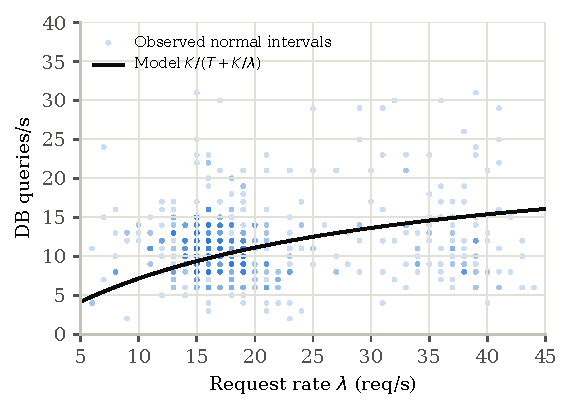
\includegraphics[width=0.62\linewidth]{figures/fig_baseline_model.pdf}
\caption{Baseline database load versus request rate. Points are normal-traffic
intervals from all sessions; the line is the analytical prediction
$q_{\mathrm{base}}=K/(T+K/\lambda)$ with $K=100$ and $T=4$~s
(Eq.~\ref{eq:baseline}).}
\label{fig:baseline-model}
\end{figure}

\subsection{Three-Condition Comparison (RQ1, RQ4)}
\label{sec:three}
Table~\ref{tab:three} reports the distribution of each metric under the three
conditions, and Figure~\ref{fig:timeline} shows one representative cycle of
normal~$\rightarrow$~undefended attack~$\rightarrow$~normal~$\rightarrow$~defended
attack.

\begin{table}[t]
\centering
\caption{Three-condition comparison on the final session. Values are median (IQR) over
sampling intervals, with p95 and maximum where informative. Failures are HTTP~503 per
second. $n$ is the number of intervals.}
\label{tab:three}
\small
\begin{tabularx}{\linewidth}{@{}L{3.3cm}YYY@{}}
\toprule
Metric & E1 Baseline & E2 Attack, undefended & E3 Attack, defended \\
& ($n=332$) & ($n=733$) & ($n=35{,}272$) \\
\midrule
Requests/s at app & 18 (16--19) & 250 (206--298) & 50 (47--53) \\
DB attempts/s & 11 (9--14) & 108 (51--150) & 6 (4--8) \\
\quad p95 / max & 17 / 34 & 205 / 317 & 12 / 174 \\
Mean latency (ms) & 77 (61--94) & 174 (101--256) & 27 (20--37) \\
\quad p95 / max & 122 / 199 & 450 / 1{,}159 & 84 / -- \\
503 failures/s & 0 (0--0) & 84 (35--124) & 0 (0--0) \\
\quad p95 / max & 0 / 3.9 & 173 / 274 & 0 / 154 \\
Intervals with any 503 & 0.3\% & 79.7\% & $<$0.01\% \\
Cache-miss ratio & 0.62 (0.50--0.75) & 0.51 (0.31--0.59) & 0.42 (0.32--0.50) \\
Coalescing ratio $\rho$ & 1.00 & 1.00 & 4.70 \\
Completed DB queries/s & 11 & 23 & 6 \\
Status & Healthy & Overloaded & Protected \\
\bottomrule
\end{tabularx}
\end{table}

\begin{figure}[t]
\centering
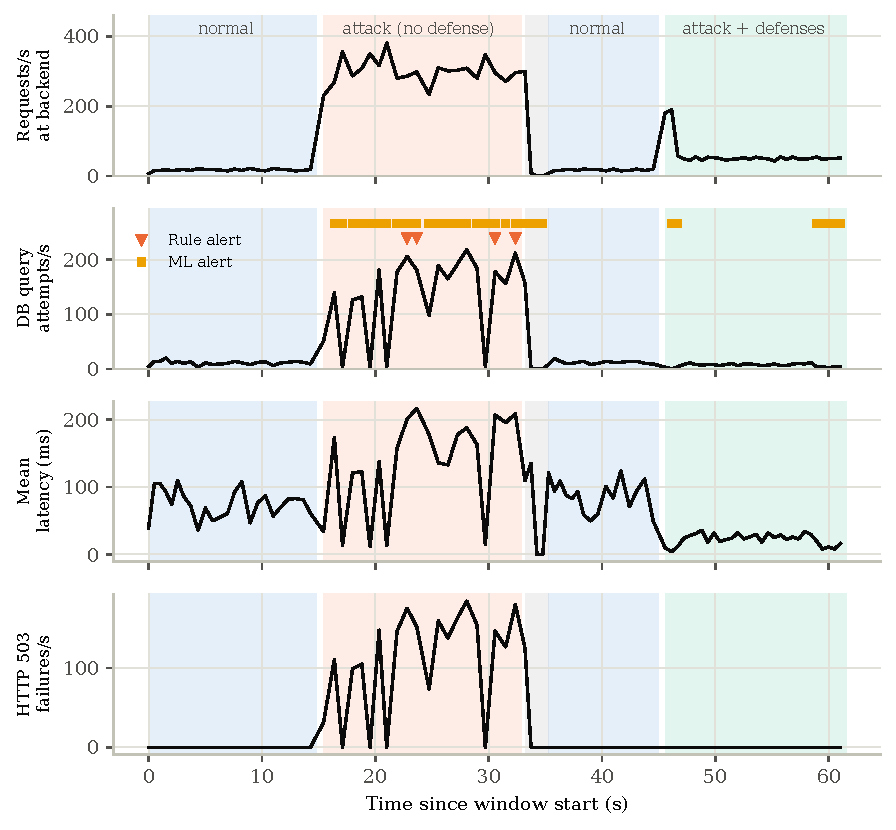
\includegraphics[width=0.92\linewidth]{figures/fig_timeline.pdf}
\caption{A representative 60~s window from the final session. Shading marks the mode
(blue: normal; orange: undefended attack; green: attack with all defenses; grey: brief
idle). Triangles and squares above the second panel mark intervals in which the rule
and the IsolationForest raised alerts.}
\label{fig:timeline}
\end{figure}

\paragraph{Undefended attack (E2).} The attack raised the application's request rate
from 18 to a median of 250~req/s and the rate of database query attempts from 11 to a
median of 108/s (9.8$\times$ the baseline median), with a peak of 317/s (28.8$\times$).
Median latency more than doubled to 174~ms, with a p95 of 450~ms and a maximum of
1.16~s, and 79.7\% of intervals contained HTTP~503 failures, at a median of 84
failures/s and up to 274/s. Of 77{,}408 database attempts, 61{,}336 (79\%) were
rejected because the pool was exhausted. This is a clear denial of service produced
entirely by well-formed requests for existing products.

\paragraph{Defended attack (E3).} With all defenses enabled, the same attack left the
database at a median of 6~q/s (IQR 4--8, p95 12)---\emph{below} the normal baseline of
11~q/s, because the edge limiter also throttles the normal traffic from the shared
load-generator address (Section~\ref{sec:validity}). The application's request rate
was pinned at the edge limiter's 50~req/s, median latency fell to 27~ms (p95 84~ms),
and failures were effectively eliminated: 419 HTTP~503 responses in 35{,}272 intervals,
concentrated in a handful of intervals at mode transitions. The defended database load
of 6~q/s is in line with the analytical bound of Eq.~\eqref{eq:defended}
($H/T=5$~q/s for the hot keys plus a small residue of normal misses).

\paragraph{Effect sizes.} The ratio of median database load, undefended to defended,
is 18.0$\times$ (95\% bootstrap CI 16.8--19.2$\times$); the ratio of means is
16.0$\times$. The ratio of median latency is 6.4$\times$ (CI 6.1--6.8$\times$).
Comparing a \emph{peak} undefended value with a \emph{typical} defended value would
give much larger factors (e.g.\ $317/6\approx53\times$); we report ratios of medians
because they are robust to the bursty, heavy-tailed behavior of the attack and are
therefore the more conservative and defensible statistic.

\paragraph{Distributions.} Figure~\ref{fig:boxplots} shows the full distributions and
Figure~\ref{fig:cdf} the latency CDFs. The defended latency distribution lies almost
entirely to the left of the baseline distribution (their interquartile ranges, 20--37~ms
and 61--94~ms, do not overlap): with stale-while-revalidate, most requests are
served from Redis in a few milliseconds, whereas in the baseline many requests are
genuine misses costing ${\geq}110$~ms. Defended service is thus not merely ``restored''
but \emph{faster than normal}, at the price of serving data up to one stale TTL old.

\begin{figure}[t]
\centering
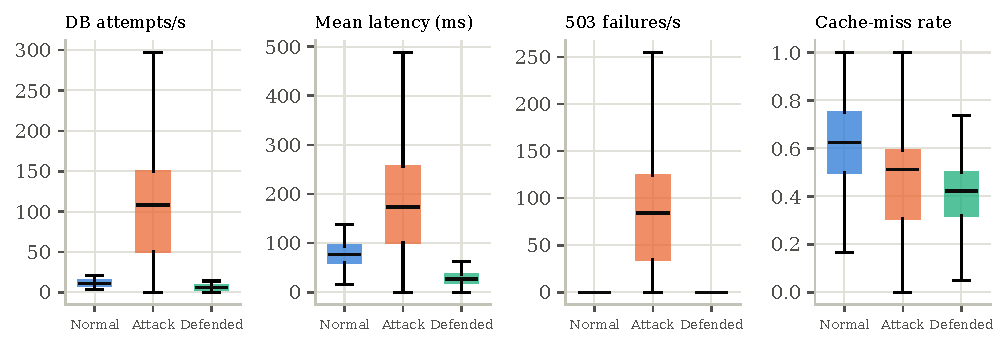
\includegraphics[width=\linewidth]{figures/fig_boxplots.pdf}
\caption{Per-interval distributions under the three conditions (final session; boxes
show IQR, whiskers 1.5$\times$IQR, outliers omitted).}
\label{fig:boxplots}
\end{figure}

\begin{figure}[t]
\centering
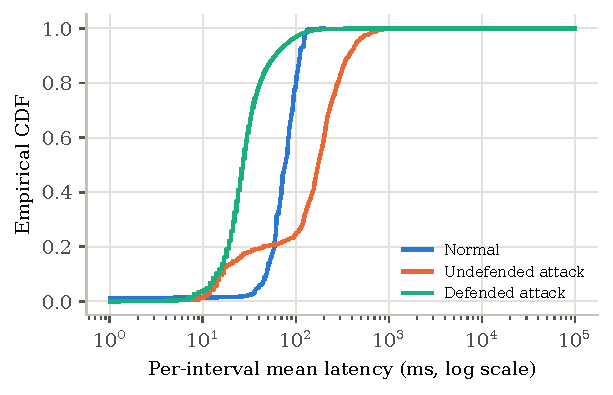
\includegraphics[width=0.66\linewidth]{figures/fig_latency_cdf.pdf}
\caption{Empirical CDF of per-interval mean latency (log scale).}
\label{fig:cdf}
\end{figure}

\paragraph{Soak test.} During the 4.5~h of valid samples in the long defended run, the
median database load was 6~q/s (p99 15), median latency 27~ms (p99 140~ms), and only a
single interval contained failures. The defense is therefore stable over hours, not
just over a demonstration-length run.

\subsection{Overload Mechanics: Why the Stampede Becomes a Denial of Service (RQ2)}
\label{sec:mechanics}
Figure~\ref{fig:saturation} plots, for every interval, the HTTP~503 rate against the
rate of database attempts. Undefended intervals lie on a line of slope close to one,
offset by roughly 20--25 attempts per second: beyond a small number of attempts per
second, \emph{every additional attempt fails}. Equivalently, the rate of
\emph{completed} database queries during the attack has a median of only 23/s---barely
twice the baseline and about one fifth of the nominal pool capacity
$\mu_{\max}=c/d_0\approx109$~q/s of Eq.~\eqref{eq:mu}.

\begin{figure}[t]
\centering
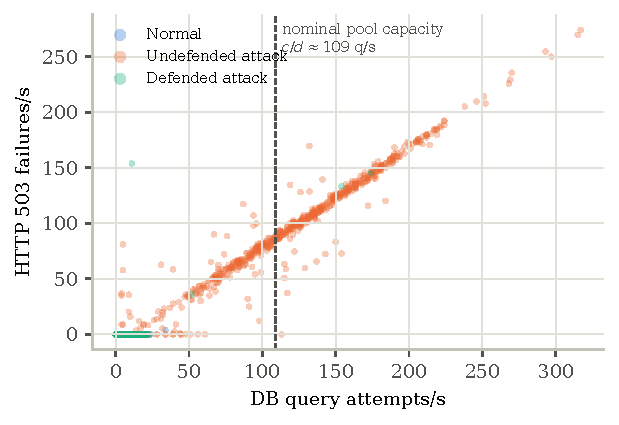
\includegraphics[width=0.66\linewidth]{figures/fig_db_saturation.pdf}
\caption{HTTP 503 failures/s versus database query attempts/s per interval. Under the
undefended attack, failures grow one-for-one with attempts once a small completed
throughput is reached, far to the left of the nominal pool capacity (dashed line).}
\label{fig:saturation}
\end{figure}

Three mechanisms, each visible in the design, explain this goodput collapse
\cite{jacobson1988,mogul1997}. First, the pool is \emph{fail-fast}
(Section~\ref{sec:bg-queueing}), so a burst of $B=250$ simultaneous misses can obtain at
most 12 connections and the rest fail at once rather than queueing. Second, failed
regenerations do not populate the cache, so a request arriving 10~ms later misses again
and makes another doomed attempt; the burst keeps re-stampeding the same key until one
query completes. Third, all 200 application threads share one Python interpreter, so
the bookkeeping of hundreds of concurrent failing requests competes for CPU with the
few that hold connections, lengthening the effective connection-holding time beyond
$d_0$. The analytical model's capacity bound is therefore optimistic by a factor of
roughly four, and the practical lesson is that \emph{the database is overwhelmed long
before its nominal capacity is reached}, because the stampede wastes the very
resource it contends for.

\subsection{Mitigation Effectiveness and Coalescing (RQ4)}
\label{sec:mitigation-results}
The coalescing ratio $\rho$ (misses per database attempt) makes the effect of locking
directly visible. Without locking, $\rho=1.00$ in both normal and attack conditions:
every miss becomes a database attempt. With locking, $\rho=4.70$ over 592{,}029 misses
and 125{,}957 database attempts: on average almost five concurrent misses were served
by one regeneration. Because losers are served the stale copy, the misses also do not
wait; the median defended latency of 27~ms is close to pure cache-hit time plus
proxy overhead. The edge limiter's effect is equally visible: the median application
request rate under attack falls from 250~req/s to exactly the configured 50~req/s.

\subsection{Mitigation Ablation}
\label{sec:ablation}
Table~\ref{tab:ablation} summarizes the ablation performed by enabling defenses one at a
time during an attack and observing the dashboard and the CacheShop storefront, and
links each step to the corresponding measured evidence.

\begin{table}[t]
\centering
\caption{Mitigation ablation (customer-visible behavior under attack). Storefront
latencies are per-item load times observed on CacheShop; DB load from the logs.}
\label{tab:ablation}
\small
\begin{tabularx}{\linewidth}{@{}L{3.4cm}L{2.5cm}L{3.1cm}L{1.8cm}Y@{}}
\toprule
Configuration & DB load & Storefront & Availability & Evidence \\
\midrule
No defense & Overloaded (median 108 attempts/s) & Fails or 300--500~ms & Denied & Table~\ref{tab:three} \\
Cache lock only (losers wait) & Protected (1--4 q/s) & Slow; up to ${\approx}2.5$~s queuing & Degraded & Bug 4, sessions 11:05--12:57 \\
+ Stale-while-revalidate & Protected & 80--140~ms, still variable & Degraded (proxy congested) & Bug 4 fix; sessions from 13:34 \\
+ Edge rate limiting & Protected (6 q/s) & 20--140~ms & Preserved & Bug 6 fix; final session \\
\bottomrule
\end{tabularx}
\end{table}

The central finding is that \emph{database protection and request-path protection are
distinct problems requiring distinct controls}. Cache locking alone protects the
database---query load drops to single digits because $N$ misses are coalesced to
one---but does not by itself keep users fast. In the first implementation losers
waited for the winner, and protected-mode latency reached ${\approx}2.5$~s;
stale-while-revalidate removed that queue. Even then, the attacker's full volume still
reached the proxy and the application: with only application-layer controls, every
attack request still consumed a proxy connection and an application thread, and the
storefront stayed slow and variable even though the database was healthy. Only edge
rate limiting, which rejects the flood at the proxy before it consumes upstream
resources, made storefront latency consistently low.

\subsection{Longitudinal Analysis of the Defense}
\label{sec:longitudinal}
Because the defense was improved during the day, the 14 sessions containing defended
traffic form a natural experiment (Figure~\ref{fig:dev}). In the first three sessions
(11:05--11:16) the median defended latency was 105--107~ms; in the next four
(11:20--12:57) 65--91~ms; from 13:34 onwards, once the stale-while-revalidate path
and real client-address forwarding were in place, it fell to 26--32~ms (42--49~ms in
two sessions that contained only defended traffic), a three- to four-fold improvement
that is stable across sessions. The lower panel shows the second
step: until the final session the application still received 170--350~req/s under a
defended attack, i.e.\ the full attack volume passed the proxy; in the final session,
with edge limiting active, it is pinned at 50~req/s. Meanwhile, undefended attacks
remained severe in every session (median latency 96--351~ms), confirming that the
improvement is due to the defense and not to a weaker attack. The first defended run
(11:05) is the only one with a substantial failure rate (146/s on average); the later
runs, and the decision recorded in the development log to count HTTP~429
(intentional shedding) separately from HTTP~503 (overload), indicate that this was an
artefact of an early version rather than a property of the defense.

\begin{figure}[t]
\centering
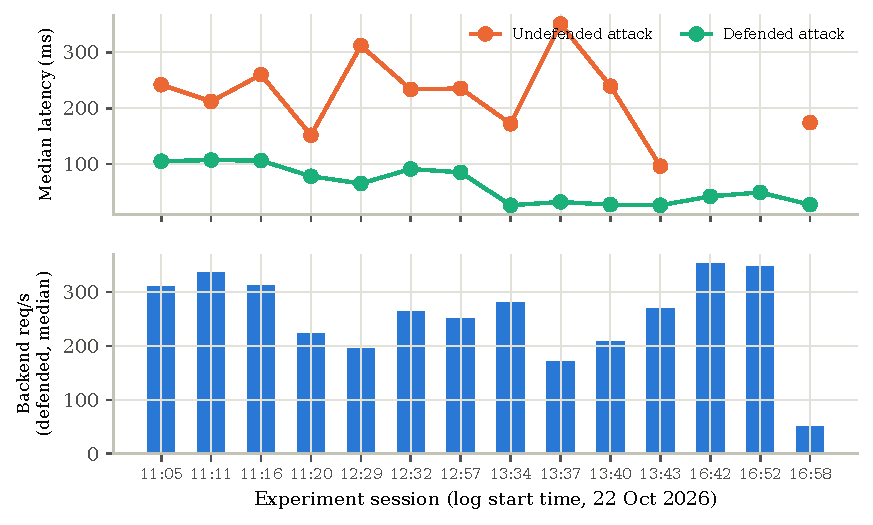
\includegraphics[width=0.92\linewidth]{figures/fig_dev_evolution.pdf}
\caption{Longitudinal view of 14 sessions. Top: median per-interval latency under
undefended and defended attack. Bottom: median request rate reaching the application
during defended attack; only in the final session does the edge limiter cap it at
50~req/s. The 16:42 and 16:52 sessions contained no undefended attack.}
\label{fig:dev}
\end{figure}

\subsection{Recovery (RQ4)}
\label{sec:recovery}
Recovery time is measured from the first interval of the new condition until the first
of two consecutive healthy intervals (Eq.~\ref{eq:healthy}). Across all sessions,
when defenses were enabled during an ongoing attack (7 transitions), the system became
healthy after a median of 1.35~s (maximum 2.77~s); in the final session the three such
transitions took 0.75, 1.35, and 1.50~s. When the attack was stopped (31 transitions),
26 recovered within the following episode, after a median of 1.08~s (maximum 2.51~s);
the remainder were followed by episodes too short to observe two healthy intervals.
Recovery is fast because cache locking immediately collapses redundant queries and the
pre-warmed stale cache serves losers without waiting, while the edge limiter's
configuration change takes effect within the watcher's one-second polling period. The
end-to-end test suite independently measured recovery after an attack stops at
${\approx}2$~s.

\subsection{Detection: Rule-Based versus IsolationForest (RQ3)}
\label{sec:det-results}

\paragraph{Per-episode detection.} Table~\ref{tab:episodes} lists the 12 undefended
attack episodes of the final session and Figure~\ref{fig:detlat} summarizes detection
latency. The rule detected 11 of 12 episodes with a median latency of 3.2~s (IQR
2.4--5.6~s, maximum 18.1~s). The IsolationForest detected 10 of 12 with a median
latency of 0.85~s (IQR 0--1.0~s, maximum 1.3~s). One ML miss occurred in the very first
attack of the session, before any normal traffic had been seen and therefore before
the model existed; the other occurred immediately after the model had been trained
for the first time on a short baseline. The two detectors' misses do not overlap, so
their union detected \emph{all 12 episodes}, with a median latency of 0.95~s.
Detection latencies of 0.0~s mean the alert was already raised in the first interval
labelled ``attack'', because traffic changes slightly before the monitor reads the new
mode flag.

\begin{table}[t]
\centering
\caption{Per-episode detection on the 12 undefended attack episodes of the final
session. $t$ = time from onset to first alert; cov.\ = fraction of the episode's
intervals with an alert; --- = not detected.}
\label{tab:episodes}
\small
\begin{tabular}{@{}rrrrrrrrr@{}}
\toprule
\# & Intervals & Duration (s) & DB med. & Latency med. & \multicolumn{2}{c}{Rule} & \multicolumn{2}{c}{IsolationForest} \\
\cmidrule(lr){6-7}\cmidrule(lr){8-9}
 & & & (q/s) & (ms) & $t$ (s) & cov. & $t$ (s) & cov. \\
\midrule
1 & 20 & 15.8 & 141 & 111 & 2.5 & 0.20 & ---$^\dagger$ & 0.00 \\
2 & 21 & 17.1 & 172 & 159 & 2.8 & 0.19 & --- & 0.00 \\
3 & 13 & 8.9 & 175 & 83 & --- & 0.00 & 0.0 & 0.31 \\
4 & 17 & 16.0 & 152 & 204 & 3.2 & 0.41 & 0.9 & 0.94 \\
5 & 21 & 16.9 & 165 & 158 & 7.4 & 0.19 & 1.0 & 0.95 \\
6 & 12 & 8.7 & 180 & 141 & 2.3 & 0.08 & 0.0 & 1.00 \\
7 & 22 & 17.5 & 188 & 142 & 1.0 & 0.09 & 1.0 & 0.95 \\
8 & 14 & 9.8 & 175 & 119 & 3.7 & 0.07 & 0.0 & 1.00 \\
9 & 65 & 53.2 & 58 & 37 & 18.1 & 0.08 & 0.8 & 0.95 \\
10 & 30 & 25.7 & 129 & 112 & 2.3 & 0.17 & 1.3 & 0.97 \\
11 & 474 & 562.1 & 100 & 209 & 3.2 & 0.35 & 0.0 & 1.00 \\
12 & 31 & 33.8 & 92 & 126 & 9.5 & 0.23 & 1.1 & 0.87 \\
\midrule
\multicolumn{5}{@{}l}{Detected / median $t$} & 11/12 & 3.2 s & 10/12 & 0.85 s \\
\bottomrule
\multicolumn{9}{@{}l}{\footnotesize $^\dagger$Model not yet trained (no normal traffic had been observed).}
\end{tabular}
\end{table}

\begin{figure}[t]
\centering
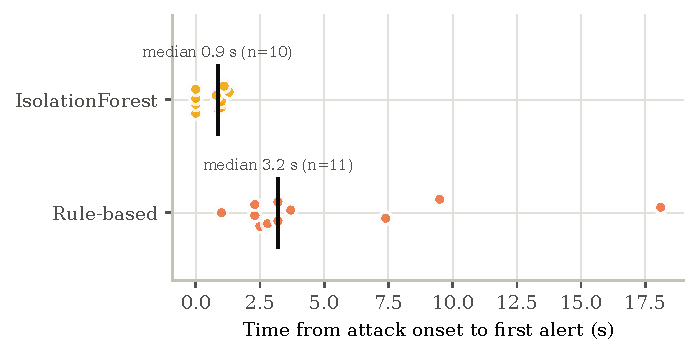
\includegraphics[width=0.66\linewidth]{figures/fig_detect_latency.pdf}
\caption{Detection latency per attack episode (final session). Vertical bars mark
medians.}
\label{fig:detlat}
\end{figure}

\paragraph{Interval-level accuracy.} Table~\ref{tab:tick} reports interval-level
metrics over 733 attack and 332 normal intervals. The rule is perfectly precise (no
false positives) but fires on only 27\% of attack intervals, because the stampede is
bursty and its three conditions coincide only intermittently. The IsolationForest
fires on 91\% of attack intervals (94\% once trained) with a single false positive in
332 normal intervals (FPR 0.3\%), giving an F1 of 0.95. Combining them with a logical
OR yields recall 0.93 and F1 0.96 at the same false-positive rate.

\begin{table}[t]
\centering
\caption{Interval-level detection performance, final session (positives: 733 attack
intervals; negatives: 332 normal intervals).}
\label{tab:tick}
\small
\begin{tabular}{@{}lrrrrrrr@{}}
\toprule
Detector & TP & FP & FN & Precision & Recall & F1 & FPR \\
\midrule
Rule (Eq.~\ref{eq:rule}) & 201 & 0 & 532 & 1.000 & 0.274 & 0.430 & 0.000 \\
IsolationForest & 670 & 1 & 63 & 0.999 & 0.914 & 0.954 & 0.003 \\
IsolationForest (model ready) & 670 & 1 & 43 & 0.999 & 0.940 & 0.968 & 0.003 \\
Rule OR IsolationForest & 678 & 1 & 55 & 0.999 & 0.925 & 0.960 & 0.003 \\
\bottomrule
\end{tabular}
\end{table}

\paragraph{Beyond attack and normal: idle and defended traffic.} Table~\ref{tab:alertrates}
shows how often each detector fires in all four modes. The rule fired in 0.01\% of
idle intervals and never in defended intervals. The IsolationForest fired in 99.3\% of
idle intervals and 12.8\% of defended intervals. The idle result is the closed-world
problem of Sommer and Paxson \cite{sommer2010} in miniature: a model that has seen only
``normal traffic'' regards \emph{no traffic} as maximally abnormal. On the dashboard
this appears as a persistent ML alert whenever traffic is stopped. The defended result
is more nuanced: during a defended attack the attack \emph{is} present, so an alert is
arguably correct as a statement about traffic, but no damage is occurring. The two
detectors are therefore answering different questions---the rule asks ``is the
database being harmed?'', the forest asks ``does traffic look unlike what I learned?''.
We return to this distinction in Section~\ref{sec:discussion}.

\begin{table}[t]
\centering
\caption{Fraction of intervals with an alert, by mode (final session).}
\label{tab:alertrates}
\small
\begin{tabular}{@{}lrrrr@{}}
\toprule
Detector & Idle ($n=25{,}586$) & Normal ($n=332$) & Attack ($n=733$) & Defended ($n=35{,}272$) \\
\midrule
Rule & 0.0001 & 0.000 & 0.274 & 0.000 \\
IsolationForest & 0.993 & 0.003 & 0.914 & 0.128 \\
\bottomrule
\end{tabular}
\end{table}

\paragraph{Why the rule is conservative: threshold sensitivity.} Figure~\ref{fig:rulegrid}
re-evaluates the rule over a grid of thresholds (with $\tau_m=0.5$). Recall is governed
almost entirely by the latency threshold $\tau_L$: at the deployed $\tau_L=200$~ms only
27\% of attack intervals qualify, while at $\tau_L=100$~ms 51\% do, and the
false-positive rate stays at or below 0.9\% everywhere on the grid. Across the full
grid (including $\tau_m$), the best F1 of 0.82 (precision 0.99, recall 0.70, FPR 0.9\%)
is obtained with $K=2$, $\tau_L=100$~ms, $\tau_m=0.3$. The deployed thresholds were
chosen during development to give zero false alarms on calm traffic and are
conservative; Figure~\ref{fig:rulegrid} shows there is room to roughly double recall at
a cost of a few false alarms per thousand intervals.

\begin{figure}[t]
\centering
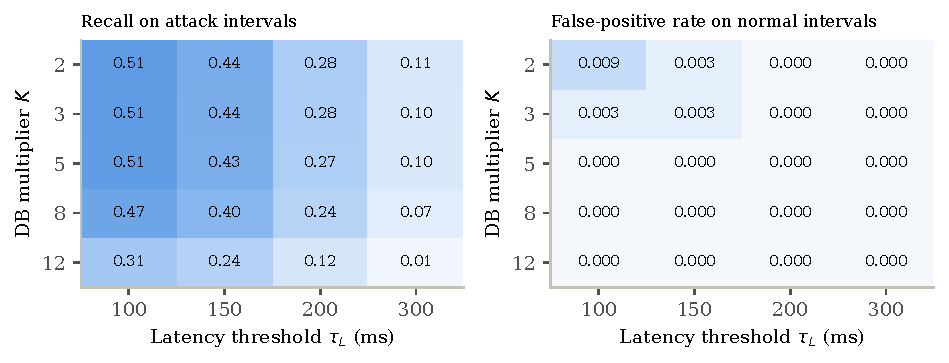
\includegraphics[width=\linewidth]{figures/fig_rule_grid.pdf}
\caption{Threshold sensitivity of the rule (final session, $\tau_m=0.5$). Left: recall
on attack intervals. Right: false-positive rate on normal intervals.}
\label{fig:rulegrid}
\end{figure}

\paragraph{Single-signal baselines and the flash-crowd proxy.} Table~\ref{tab:single}
evaluates each signal alone. On the attack/normal intervals, a pure volume threshold
(rps$\,>100$) looks excellent (recall 0.97, no false positives), because in this
testbed attack traffic is an order of magnitude larger than normal traffic. Its
weakness appears on the 2{,}080 absorbed-burst intervals, in which the full attack
volume reached the application but was served from cache: the volume detector fired on
97.1\% of them, whereas the database-load condition, the failure condition, and the
full rule fired on none. This is the quantitative justification for the multi-signal
design: \emph{volume detects traffic; the rule detects harm}. The table also exposes a
weakness in the rule's third condition. Because the normal miss ratio is already high
(Section~\ref{sec:baseline}), ``miss ratio $>0.5$'' fires on 67\% of normal intervals
and, on its own, is worse than useless; within the conjunction it only removes true
positives. The database-load condition alone (F1 0.85) and the presence of 503 failures
(F1 0.89) are each stronger than the full three-way rule as deployed.

\begin{table}[t]
\centering
\caption{Single-signal detectors versus the rule. Left: attack (positive) vs.\ normal
(negative) intervals, final session. Right: fraction of 2{,}080 absorbed-burst
intervals (high volume, served from cache, no harm) on which the detector fires.}
\label{tab:single}
\small
\begin{tabular}{@{}lrrrr|r@{}}
\toprule
Detector & Precision & Recall & F1 & FPR & Fires on absorbed bursts \\
\midrule
Volume: rps $>100$ & 1.000 & 0.966 & 0.983 & 0.000 & 97.1\% \\
DB load $>5\times$ baseline & 1.000 & 0.739 & 0.850 & 0.000 & 0.0\% \\
Mean latency $>200$ ms & 1.000 & 0.404 & 0.575 & 0.000 & 0.8\% \\
Miss ratio $>0.5$ & 0.636 & 0.531 & 0.578 & 0.672 & 8.3\% \\
Any 503 failures & 0.998 & 0.797 & 0.886 & 0.003 & 0.0\% \\
DB load AND miss ratio & 1.000 & 0.516 & 0.680 & 0.000 & 0.0\% \\
Rule (all three) & 1.000 & 0.274 & 0.430 & 0.000 & 0.0\% \\
\bottomrule
\end{tabular}
\end{table}

\paragraph{Offline IsolationForest analysis.} Re-running the ML pipeline offline
(trained on 166 normal intervals, tested on 166 held-out normal and 733 attack
intervals) gives a ROC AUC of 0.999 (Figure~\ref{fig:roc}); across ten random seeds
the AUC ranged from 0.994 to 1.000. The ranking quality of the five-feature score is
excellent and stable; what varies is the operating point. Table~\ref{tab:contam} shows
the effect of the \texttt{contamination} parameter: at the deployed value of 0.01 the
model reaches recall 0.989 at a held-out false-positive rate of 1.8\%, while raising it
to 0.03 buys perfect recall at an FPR of 11.5\%---an unacceptable alarm rate for a
signal evaluated twice per second. Among single features, request rate alone is
almost as good a ranking score as the full model (AUC 0.995), again reflecting the
large volume difference in this testbed; the miss ratio has an AUC of 0.25, i.e.\ it is
\emph{inversely} related to the attack, consistent with Table~\ref{tab:three}.

\begin{figure}[t]
\centering
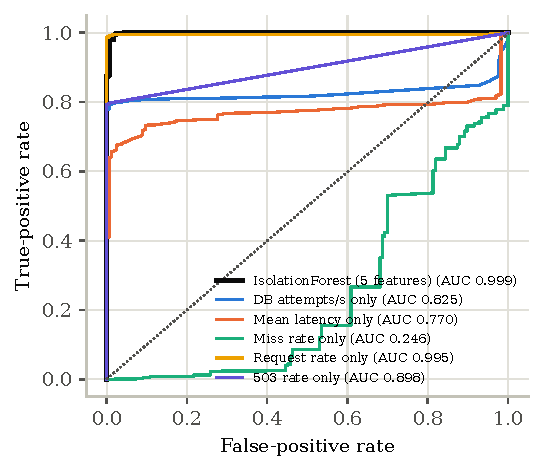
\includegraphics[width=0.56\linewidth]{figures/fig_roc.pdf}
\caption{ROC curves on held-out normal and attack intervals for the offline
IsolationForest and for each of its input features used alone as a score.}
\label{fig:roc}
\end{figure}

\begin{table}[t]
\centering
\caption{Offline IsolationForest: effect of the contamination parameter and of the
training-window size (test: 166 normal, 733 attack intervals).}
\label{tab:contam}
\small
\begin{tabular}{@{}lrrrr@{\hspace{2.2em}}lrrr@{}}
\toprule
\multicolumn{5}{@{}c}{Contamination (train $n=166$)} & \multicolumn{4}{c@{}}{Training size (contam.\ 0.01)} \\
\cmidrule(r{2.2em}){1-5}\cmidrule(l){6-9}
Value & Precision & Recall & FPR & AUC & $n$ & Recall & FPR & F1 \\
\midrule
0.01 & 0.996 & 0.989 & 0.018 & 0.999 & 10 & 0.156 & 0.012 & 0.269 \\
0.03 & 0.975 & 1.000 & 0.115 & 0.999 & 20 & 0.903 & 0.024 & 0.946 \\
0.05 & 0.959 & 1.000 & 0.187 & 0.999 & 50 & 0.874 & 0.042 & 0.928 \\
0.10 & 0.943 & 1.000 & 0.265 & 0.999 & 100 & 0.218 & 0.000 & 0.358 \\
     &       &       &       &       & 166 & 0.989 & 0.018 & 0.992 \\
\bottomrule
\end{tabular}
\end{table}

The training-size sweep reveals the detector's main fragility. With the first 10
normal intervals---the deployed minimum---recall on the held-out attack set is only
0.16; with 20 it is 0.90; but with 100 it falls back to 0.22 before recovering to 0.99
with all 166. The forest's decision threshold is set from the training scores, so its
operating point depends on which particular normal intervals happen to be in the
window (for example, whether a brief high-latency normal interval is present). This
non-monotonic behavior explains the one ``ready but silent'' ML miss in
Table~\ref{tab:episodes}, and argues for a longer minimum training window and for
fixing the decision threshold on a validation set rather than through
\texttt{contamination} alone.

\paragraph{Summary for RQ3.} The two detectors are complementary rather than
interchangeable. The IsolationForest is fast (sub-second median), dense (recall 0.91),
and adaptive, but depends on a clean, sufficiently long training window and flags any
departure from what it has seen, including idleness. The rule is slower and sparser
but perfectly precise, interpretable, available from the first second, and---because
it measures harm rather than novelty---silent on both absorbed bursts and defended
attacks. Together they detected every attack with one false alarm.

\subsection{End-to-End Validation}
\label{sec:validation}
The automated suite \texttt{tests/test\_cachecollapse.py} drives the live stack through
the same control API as the dashboard and samples the SSE feed. Its final run passed
all 16 cases (Table~\ref{tab:tests}). Its quantitative evidence---for example a peak of
227 DB q/s and 145 failures per interval under attack versus 11 q/s and none with
protection, and 20 of 20 storefront requests succeeding during a defended
attack---agrees with the log analysis above.

\begin{table}[t]
\centering
\caption{End-to-end test suite (final run: 16/16 passed).}
\label{tab:tests}
\small
\begin{tabularx}{\linewidth}{@{}rL{6.0cm}Y@{}}
\toprule
\# & Test & Evidence recorded \\
\midrule
1 & All 9 containers running & 9 up \\
2 & Dashboard page loads & HTTP 200, correct title \\
3 & Storefront loads & HTTP 200, ``CacheShop'' present \\
4 & Product API returns data & \texttt{/api/products/1} $\rightarrow$ 200 with name and price \\
5 & Cache works (second call faster) & 137 ms (DB) $\rightarrow$ 9 ms (cache) \\
6 & Unknown product returns 404 & \texttt{/api/products/99999} $\rightarrow$ 404 \\
7 & Baseline is calm & Peak DB 17 q/s; 0 alerts \\
8 & Attack overloads the DB & Peak latency 500 ms, DB 227 q/s, 145 failures per interval \\
9 & Rule detector fires on attack & 10 samples alerted \\
10 & ML detector fires on attack & 28 samples alerted \\
11 & Cache locking keeps DB load low & Peak DB 11 q/s (vs.\ 227 undefended) \\
12 & Protection preserves availability & Peak latency 152 ms, 0 failures \\
13 & System recovers after attack stops & Healthy again in ${\approx}2$ s \\
14 & Live feed updates faster than 1 s & Two samples 0.6 s apart differ \\
15 & Control endpoints respond & traffic / attack / defense / reset OK \\
16 & Storefront served while protected & 20/20 product requests succeed under attack + defense \\
\bottomrule
\end{tabularx}
\end{table}
